%% Copernicus Publications Manuscript Preparation Template for LaTeX Submissions
%% ---------------------------------
%% This template should be used for the following class files: copernicus.cls, copernicus2.cls, copernicus_discussions.cls
%% The class files, the Copernicus LaTeX Manual with detailed explanations regarding the comments
%% and some style files are bundled in the Copernicus Latex Package which can be downloaded from the different journal webpages.
%% For further assistance please contact the Publication Production Office (production@copernicus.org).
%% http://publications.copernicus.org


%% Differing comments regarding the specific class files are highlighted.


%% copernicus.cls
\documentclass[acp]{copernicus}

%% copernicus2.cls
%\documentclass[acp]{copernicus2}

%% copernicus_discussions.cls
%\documentclass[journal abbreviation, hvmath, online]{copernicus_discussions}


\begin{document}


\title{Entrainment and detrainment rates of individual shallow cumulus clouds 
in a LES}


\author[1]{Jordan T Dawe}
\author[1]{Philip H Austin}

\affil[1]{Department of Earth and Ocean Sciences, 
        University of British Columbia, 
	6339 Stores Road, 
        Vancouver, BC, 
        V6T 1Z4}

%% The [] brackets identify the author to the corresponding affiliation, 1, 2, 3, etc. should be inserted.



\runningtitle{ENTRAINMENT}

\runningauthor{Dawe and Austin}

\correspondence{Jordan T Dawe\\ (jdawe@eos.ubc.ca)}



\received{}
\pubdiscuss{} %% only important for two-stage journals
\revised{}
\accepted{}
\published{}

%% These dates will be inserted by the Publication Production Office during the typesetting process.


\firstpage{1}

\maketitle



\begin{abstract}
TK
\end{abstract}


%% only used for copernicus2.cls
%\abstract{
% TEXT
% \keywords{TEXT}}



\introduction
%% \introduction[modified heading if necessary]

TEXT TK

%==============================================================================

\section{Model Description}

All LES calculations in this paper were made using the System for Atmospheric 
Modeling \citep[SAM;][]{Khairoutdinov2003}.  SAM is an anelastic LES 

The model was run configured as standard Global Energy and Water
Cycle Experiment (GEWEX) Cloud System Studies \citep[GCSS;][]{Randall2003}
Barbados Oceanographic and Meteorological Experiment 
\citep[BOMEX;][]{Siebesma2003} experiment.  BOMEX simulates a trade-wind cumulus 
cloud field observed over ocean near Bermuda

The BOMEX run was performed on a 6.4 km x 6.4 km horizontal x 3.2 km vertical 
domain with 25 meter grid resolution in all directions for 6 hours, and the 
first three hours of simulation were discarded. 

%==============================================================================

\section{A Taxonomy of Entrainment and Detrainment}

TK

%==============================================================================

\section{Cloud field height-area}


%==============================================================================

\section{Entrainment Histograms}

TK

%==============================================================================

\section{Corrected Entrainment and Detrainment}

Consider a numerical model grid cell containing a cloud surface with normal 
vector $\mathbf{C}$, where $\mathbf{C}$ points outward from the surface and 
has units of m$^2$ (Figure TK).  This surface, 
combined with $\mathbf{W}$, the portion of the grid cell walls that lie within 
the cloud in m$^2$, encloses a cloud volume $V$ which has units of m$^3$.  
\cite{Siebesma1998} gives the net entrainment and detrainment over the cloud 
surface to be:
\begin{equation}
\label{eq:E_minus_D} 
E - D = \int_C \rho \phi ( \mathbf{u_i} -  \mathbf{u}) \cdot d\mathbf{C},
\end{equation}
where $\rho$ is the air density in kg m$^{-3}$, $\mathbf{u}$ is the velocity
of the air in m s$^{-1}$ and $\mathbf{u_i}$ is the velocity of the cloud 
interface in m s$^{-1}$.  Calculating this integral requires knowledge of the 
velocity field over the surface of $\mathbf{C}$ and the time evolution of 
$\mathbf{C}$, neither of which is easily calculated in a numerical model.  
Instead, we seek a simplified but equivalent calculation.

To calculate the velocity of the cloud surface, we make use of the Leibnitz 
Theorem:
\begin{equation}
\label{eq:leibnitz} 
\frac{d}{dt}\int_{V(t)} \rho \phi dV = 
  \int_{V(t)} \frac{\partial \rho \phi}{ \partial t} dV 
  + \int_{C(t)} \rho \phi \mathbf{u_i}\cdot d\mathbf{C}
  + \int_{W(t)} \rho \phi \mathbf{u_i}\cdot d\mathbf{W}.
\end{equation}
Since the walls of the grid cell do not move, $\mathbf{u_i}$ is 0 over 
$\mathbf{W}$.  If we also assume ${\partial \rho}/{ \partial t} \approx 0$, we
get
\begin{equation}
\label{eq:leibnitz2} 
    \rho \frac{d}{dt}\int_{V(t)} \phi dV = 
    \int_{V(t)} \rho \frac{\partial \phi}{ \partial t} dV 
    \int_{C(t)} \rho \phi \mathbf{u_i}\cdot d\mathbf{C}.
\end{equation}
We then combine equations (\ref{eq:E_minus_D}) and (\ref{eq:leibnitz2}) to give:
\begin{equation}
\label{eq:step1} 
      E - D = \rho \frac{d}{dt}\int_{V(t)} \phi dV
            - \int_{V(t)} \rho \frac{\partial \phi}{ \partial t} dV 
            - \int_C \rho \phi \mathbf{u} \cdot d\mathbf{C}.
\end{equation}

Next we apply the divergence theorem to simplify the flux integral through 
$\mathbf{C}$:
\begin{equation}
\label{eq:divergence} 
\int_{V} \nabla \cdot (\rho \phi \mathbf{u}) dV = 
  \int_{C} \rho \phi \mathbf{u}\cdot d\mathbf{C}
+ \int_{W} \rho \phi \mathbf{u}\cdot d\mathbf{W}
\end{equation}

Substituting this into (\ref{eq:step1}) results in
 \begin{equation}
\label{eq:entrainment_detrainment} 
E - D = \rho \phi \frac{dV}{dt} 
  - V \nabla \cdot (\rho \phi \mathbf{u})
  + \int_W \rho \phi \mathbf{u} \cdot d\mathbf{W}.
\end{equation}
Following \cite{Romps2010}, if (\ref{eq:entrainment_detrainment}) is positive,
the result of this calculation is assumed to all be $E$, and if negative, $D$: 

\begin{equation}
\label{eq:max_ent} 
E = \mathrm{max}\left(0, 
    \rho \phi \frac{dV}{dt}
  - V \nabla \cdot (\rho \phi \mathbf{u})
  + \int_W \rho \mathbf{u} \cdot d\mathbf{W}\right)
\end{equation}
\begin{equation}
\label{eq:max_det} 
D = \mathrm{max}\left(0, 
  - \rho \phi \frac{dV}{dt} 
  + V \nabla \cdot (\rho \phi \mathbf{u})
  - \int_W \rho \mathbf{u} \cdot d\mathbf{W}\right).
\end{equation}
Therefore, we can find the entrainment and detrainment by calculating the rate 
of change of the cloud volume inside the grid cell and the mass flux through 
the cloudy portion of the grid cell 



%==============================================================================

* $\chi_q$ calculation: *

\begin{equation}
\chi_q = \frac{(1 + \gamma) q_l}{\Delta q_t - \pi \Delta \theta_l \frac{\partial q_s}{\partial T}}
\end{equation}



%==============================================================================

\conclusions
%% \conclusions[modified heading if necessary]

TK


\appendix
\section{\\ \\ \hspace*{-7mm} Calculation of the Density Potential Temperature Lapse Rate}    %% Appendix A

To calculate the density lapse rate, we start with the density potential 
temperature, which is given approximately by:

\begin{equation}
\label{eq:density_potential_temperature}
  \theta_\rho(T, p, q_v, q_l) = T \left(\frac{p_o}{p}\right)^\gamma (1 + \lambda q_v - q_l)
\end{equation}

If we assume the parcel is saturated, we can replace $q_v$ with $q_s(T, p)$ and 
$q_l$ with $q_t - q_s(T, p)$, giving:

\begin{equation}
\label{eq:density_potential_temperature_qs}
  \theta_\rho(T, p, q_s) = T \left(\frac{p_o}{p}\right)^\gamma (1 + (\lambda + 1) q_s(T, p) - q_t)
\end{equation}


Taking the derivative of this with height gives:

\begin{equation}
\label{eq:density_potential_temperature_gradient_1}
  \frac{d \theta_\rho}{dz} = \frac{\partial \theta_\rho}{\partial T}\frac{dT}{dz}
                          + \frac{\partial \theta_\rho}{\partial p}\frac{dp}{dz}
                          + \frac{\partial \theta_\rho}{\partial q_s}\frac{dq_s}{dz}
\end{equation}

The partial derivatives of $\theta_\rho$ are given by:
\begin{equation}
  \frac{\partial \theta_\rho}{\partial T} = \frac{\theta_\rho}{T}
\end{equation}
\begin{equation}
  \frac{\partial \theta_\rho}{\partial p} = -\gamma \frac{\theta_\rho}{p}
\end{equation}
\begin{equation}
  \frac{\partial \theta_\rho}{\partial q_s} = \frac{(\lambda + 1)\theta_\rho}{(1 + (\lambda + 1)q_s - q_t)}
\end{equation}

For the last of these partial derivatives, we note that 
$(1 + (\lambda + 1)q_s - q_t) \approx 1$ and write

\begin{equation}
  \frac{\partial \theta_\rho}{\partial q_s} \approx (\lambda + 1) \theta_\rho 
\end{equation}

As $q_s$ is a function of $T$ and $p$, we must expand its derivative as 
well:

\begin{equation}
\label{eq:q_s_derivative}
  \frac{d q_s}{dz} = \frac{\partial q_s}{\partial T}\frac{dT}{dz}
                          + \frac{\partial q_s}{\partial p}\frac{dp}{dz}
\end{equation}

Putting all these expansions together gives:

\begin{equation}
\label{eq:density_potential_temperature_gradient_2}
  \frac{d \theta_\rho}{dz} = \theta_\rho \left[ 
                               \left( \frac{1}{T} + (\lambda + 1)\frac{\partial q_s}{\partial T} \right)\frac{dT}{dz}
                             + \left( -\frac{\gamma}{p} + (\lambda + 1)\frac{\partial q_s}{\partial p} \right)\frac{dp}{dz}
                             \right]
\end{equation}

$dT/dz$ is simply the moist adiabatic lapse rate $\Gamma_m$, given 
approximately by:
\begin{equation}
\Gamma_m = g\frac{1 + \frac{L_v q_v}{R_d T}}{c_p + \frac{L_v^2 q_v \epsilon}{R_d T^2}}
\end{equation}
$dp/dz$ can be calculated from the model mean state, and 
$\partial q_s/\partial T$ and $\partial q_s/\partial p$ are given
by empirical formulae.


%\subsection                               %% Appendix A1, A2, etc.

\begin{acknowledgements}
Support for this research was provided by the Canadian Foundation for Climate 
and Atmospheric Science through the Cloud Aerosol Feedback and Climate 
network. We thank Marat Khairoutdinov for making SAM available to the cloud 
modeling community. Figures were generated using the matplotlib library in the 
Python programming language.
\end{acknowledgements}


\bibliographystyle{copernicus}
\bibliography{./bibliography/entrainment}


%% Literature citations
%% command                        & example result
%% \citet{jones90}|               & Jones et al.\ (1990)
%% \citep{jones90}|               & (Jones et al., 1990)
%% \citep{jones90,jones93}|       & (Jones et al., 1990, 1993)
%% \citep[p.~32]{jones90}|        & (Jones et al., 1990, p.~32)
%% \citep[e.g.,][]{jones90}|      & (e.g., Jones et al., 1990)
%% \citep[e.g.,][p.~32]{jones90}| & (e.g., Jones et al., 1990, p.~32)
%% \citeauthor{jones90}|          & Jones et al.
%% \citeyear{jones90}|            & 1990






%% FIGURES %%%%%%%%%%%%%%%%%%%%%%%%%%%%%%%%%%%%%%%%%%%%%%%%%%%%%%%%%%%%%%%%%%%%


%% ONE-COLUMN FIGURES

%f
%\begin{figure}[t]
%\vspace*{2mm}
%\begin{center}
%\includegraphics[width=8.3cm]{./figures/figure1}
%\end{center}
%\caption{Schematic representation of our cloudlet algorithm.}
%\label{fig:cloudfinder_instructions}
%\end{figure}


%% TWO-COLUMN FIGURES

%f
%\begin{figure*}[t]
%\vspace*{2mm}
%\begin{center}
%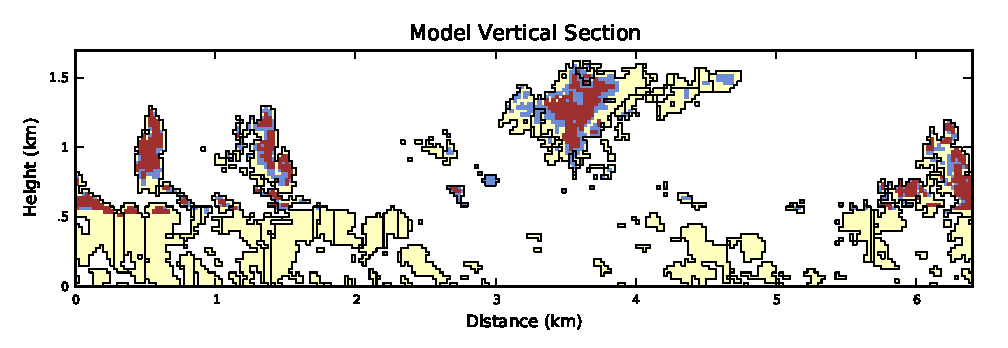
\includegraphics[width=\textwidth]{./figures/vertical_section}
%\end{center}
%\caption{Vertical section through the BOMEX model, showing the cloud core
%(black), the cloud (dark grey) and the plume (light grey) regions used by the 
%cloud tracking algorithm.}
%\label{fig:cloudfinder_instructions}
%\end{figure*}


%% TABLES %%%%%%%%%%%%%%%%%%%%%%%%%%%%%%%%%%%%%%%%%%%%%%%%%%%%%%%%%%%%%%%%%%%%


%% ONE-COLUMN TABLE

%t
%\begin{table}[t]
%\caption{Statistics of tracked clouds}
%\vskip4mm
%\centering
%\begin{tabular}{llcr}
%\tophline
%&&BOMEX\\
%\middlehline
%Total Clouds&&1183\\
%Starts\\
%&Broken&59\\
%&Split&339\\
%&New&785\\
%Ends\\
%&Broken&39\\
%&Merge&51\\
%&Decay&1093\\

%\bottomhline
%\end{tabular}
%\end{table}

%% TWO-COLUMN TABLE

\begin{table*}[t]
\caption{Taxonomy of cloud core entrainment and detrainment}
\vskip4mm
\centering
\begin{tabular}{llccc}
\tophline
& Process & $q_l$ & $\theta_v - \overline{\theta_v}$ & $w$\\

\middlehline
Entrainment & & & & \\
& Adiabatic Processes & + & + & + \\
& Environmental Buoyancy Change & - & - & - \\
& Mixing & + & + & + \\
& Radiation & - & + & - \\

\middlehline
Detrainment & & & & \\
& Adiabatic Pressure Change & - & - & - \\
& Environmental Buoyancy Change & - & + & - \\
& Mixing & + & + & + \\
& Radiation & + & + & - \\


\bottomhline
\end{tabular}
\end{table*}

%% The different columns must be seperated with a & command and should
%% end with \\ to identify the column brake.

%%%%%%%%%%%%%%%%%%%%%%%%%%%%%%%%%%%%%%%%%%%%%%%%%%%%%%%%%%%%%%%%%%%%%%%%%%%%%%


%% If figures and tables must be numbered 1a, 1b, etc. the following command
%% should be inserted before the begin{} command.

%\addtocounter{figure}{-1}\renewcommand{\thefigure}{\arabic{figure}a}


\end{document}
